\documentclass{article}
\usepackage{style}
\begin{document}
\maketitle
\tableofcontents
\section{Introducción}
La representación del individuo es el primer componente del algoritmo genético, el cual representa soluciones potenciales al problema. La representación más tradicional es la binaria, la cual fue propouesta por Holland ya que tenía un grado elevado de paralelismo implícito, pero esta implica varias desventajas para dar soluciones para problemas del mundo real, por ende se han creado diferentes representaciones como la binaria la real y la de gray.
\section{Contenido}
\subsection{Ejemplo de representación binaria}
\begin{figure}[h!]
	\centering
	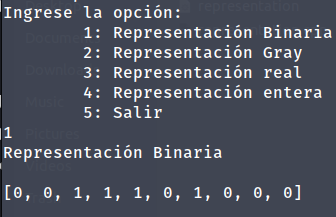
\includegraphics[scale=.6]{binary}
\end{figure}
\newpage
\subsection{Ejemplo de representación en código gray}
\begin{figure}[h!]
	\centering
	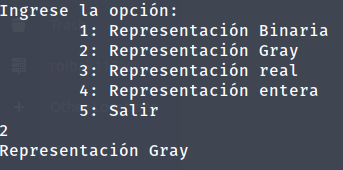
\includegraphics[scale=.7]{gray}
\end{figure}
\subsection{Ejemplo de representación real}
\begin{figure}[h!]
	\centering
	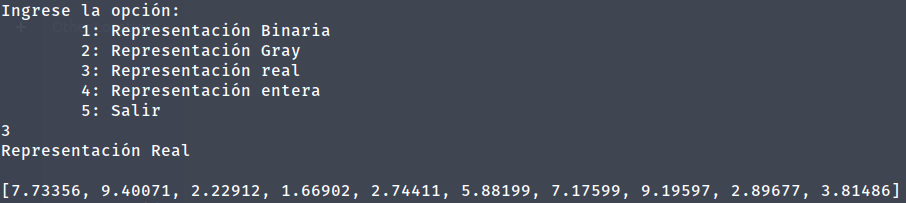
\includegraphics[scale=.5]{real}
\end{figure}
\subsection{Ejemplo de representación entera}
\begin{figure}[h!]
	\centering
	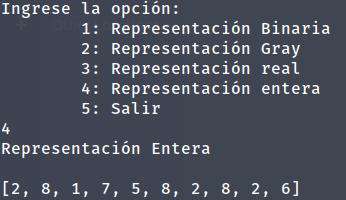
\includegraphics[scale=.7]{integer}
\end{figure}
\section{Conclusión}
Las diferentes representaciones tienen sus ``tradeoffs'', dependiendo del problema a resolver se elige una de ellas.
\end{document}